\section{Wirkungsplan}
Aus der folgenden Differentialgleichung ist das System mit Simulink zu
modellieren.
\[
	\dot{\omega}(t)
		+ \frac{1}{J} \left(\alpha + \frac{K^2}{R}\right) \omega(t)
	= \frac{K}{JR} u(t) - \frac{1}{J} \Gamma_l(t)
\]

\subsection{Formale Analyse}
Hierbei handelt es sich um eine lineare Differentialgleichung erster Ordnung.
Hierzu muss die Differentialgleichung zuert in die Richtige Form gebracht
werden. In einem ersten Schritt wird die Differentialgleichung explizit nach
der höchsten Ableitung dargestellt.
\[
	\dot{\omega}(t)
	= - \frac{1}{J} \left(\alpha + \frac{K^2}{R} \right) \omega(t)
		+ \frac{K}{JR} u(t) - \frac{1}{J} \Gamma_l(t)	
\]
Diese Differentialgleichung wird nun integriert nach der Zeit $t$, da $\omega$
eine Funktion der Zeit ist.
\[
	\omega(t)
	= - \frac{1}{J} \left(\alpha + \frac{K^2}{R} \right) \int\omega(t)\,dt
		+ \frac{K}{JR} \int u(t)\,dt
		- \frac{1}{J} \int \Gamma_l(t)\,dt
\]
Diese Form der Differentialgleichung zeigt, dass die Ausgangsgrösse des
Systems aus drei Summanden zusammengesetzt ist, wobei jeder dieser Summanden
eine Integration nach der Zeit $t$ aufweist. Bei einer dieser Grössen ist
die Ausgangsgrösse selbt integriert und zurückgeführt. Offensichtlich ist dies
das Feedback des Systems.

\subsection{Implementierung in MATLAB/Simulink}
Um dieses System in MATLAB bzw. Simulink übersichtlicher aufzubauen werden
die Konstanten Terme wie folgt substituiert.
\[
	\omega(t)
	= \underbrace{- \frac{1}{J} \left(\alpha + \frac{K^2}{R} \right)}_{x}
		\int\omega(t)\,dt
		\underbrace{+ \frac{K}{JR}}_{y} \int u(t)\,dt
		\underbrace{- \frac{1}{J}}_{z} \int \Gamma_l(t)\,dt
\]
Da in der Aufgabenstellung keinerlei Werte weder für die Konstanten gegeben
sind noch für die Funktionene, werden die folgenden Annahmen getroffen:
\begin{itemize}
	\item alle Konstanten ($\alpha$, $J$, $K$, $R$) haben den Wert 1
	\item das Lastmoment wird als konstant angenommen mit dem Wert 0
	\item die Spannung ($u(t)$) ist eine Sprungfunktion mit Amplitude 1
\end{itemize}

\lstinputlisting{../../matlab/exercise/ex_01/ex_01_init.m}

\begin{figure}[h!]
	\centering
	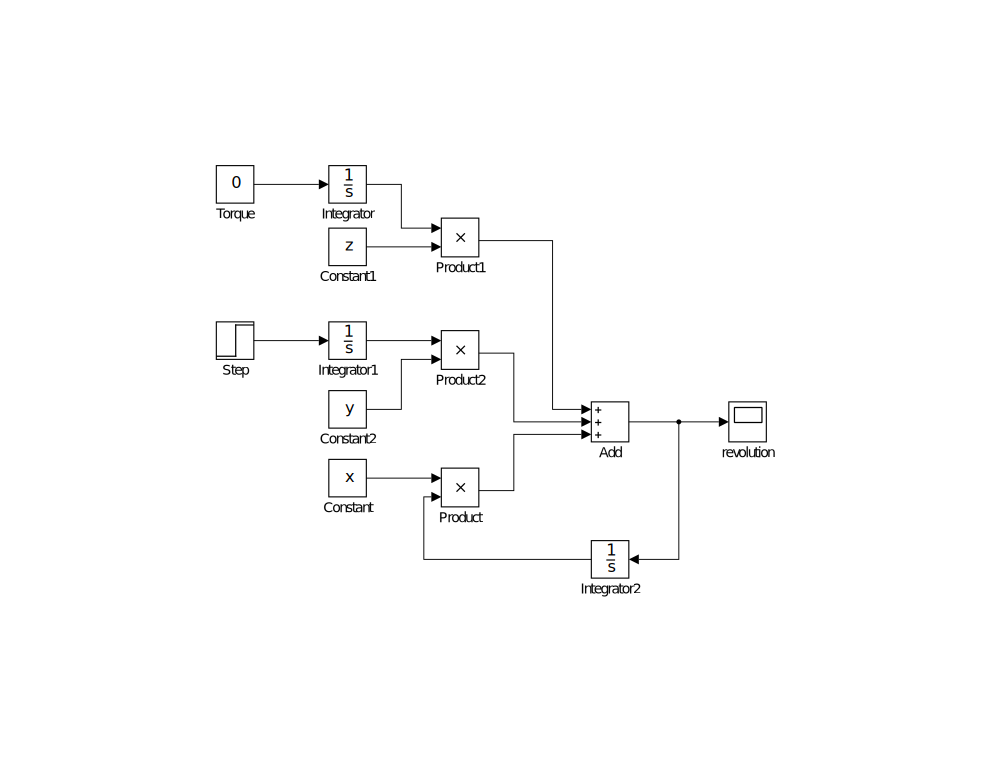
\includegraphics[width=1\textwidth]{../../matlab/exercise/ex_01/ex_01.pdf}
	\caption{Simulink-Model}
\end{figure}

\subsection{Plausibilitätsprüfung}
Um die plausibilität des Modells zu prüfen weden spezifische Zustände geprüft.

\subsubsection{Unbelastete Welle}
Wird der Motor mit positiver Spannung und ohne Lastmoment betireben, so muss
sich eine positive Drehzahl einstellen. Die Motorspannung ist mit einer
Sprungfunktion gegeben mit der Amplitude 1. Die Simulation zeigt, dass sich
eine Drehzahl von 5 einstellt.

\subsubsection{Belastete Welle}
Liegt ein positives Lastmoment an, wobei keine Spannung anliegt, so muss sich
eine negative Drehzahl einstellen. Für diese Prüfung ist ein Lastmoment
$\Gamma(t) = const. = 1$ gewählt worden. Die Simulation zeigt, dass sich eine
Drehzahl von -0.5 einstellt.

\subsubsection{Überbelastete Welle}
Wird der Motor mit einem grossen Lastmoment belastet, so muss sich eine
negative Drehzahl einstellen. Das Lastmoment ist konstant gewählt als
$\Gamma(t) = const. = 10$ und die Motorspannung ist als Sprungfunktion
gegeben mit der Amplitude 5. Die Simulation zeigt, dass sich vor dem Sprung
eine Drehazhl von -5 einstellt durch das Lastmoment. Nach den Sprung
resultiert eine Drehzahl von -2.5 durch das entgegenwirken des Motors.

\subsubsection{Anfangsbedingung $\omega(t=0) \neq 0$}
Liegt weder ein Lastmoment an der Welle noch eine Spannung am Motor, so muss
sich die Drehzahl für die Anfangsbedingung $\omega(t=0) \neq 0$ gegen 0
annähern. Die Simulation zeigt, dass sich die Drehzahl gegen 0 annähert mit
der Zeit. Dies gilt sowohl für positive als auch negative Anfangsbedingungen.

\subsubsection{Sinus als Eingangsfunktion}
Wird eine Sinusfunktion für die Motorspannung gewählt, so muss sich auch
eine Sinusgrösse am Ausgang einstellen. Dies muss für jedes anliegende
Lastmoment an der Welle gelten. Die Simulationen haben gezeigt, dass sich
für alle Lastmomente eine Sinusförmige Drehzahl ergibt für eine Sinusförmige
Motorspannung. der Offset der Sinuskurve am Ausgang ist dabei gegeben durch
das anliegenede Lastmoment.

\subsubsection{Fazit}
Die Plausibilitätsprüfungen deuten darauf hin, dass das modellierte System
sich wie erwartet verhält.
